\documentclass{article}
\usepackage[top=1in, bottom=1in, left=1in, right=1in]{geometry}
\usepackage[dvipsnames]{xcolor}
\usepackage{amsmath, amssymb, amsthm}
\usepackage{graphicx}

\newcommand{\EE}{\mathbb{E}}
\newcommand{\PP}{\mathbb{P}}
\newcommand{\Dd}{\mathcal{D}}
\newcommand{\Ee}{\mathcal{E}}
\newcommand{\Hh}{\mathcal{H}}
\newcommand{\Ll}{\mathcal{L}}
\newcommand{\Ss}{\mathcal{S}}
\newcommand{\Xx}{\mathcal{X}}
\newcommand{\Yy}{\mathcal{Y}}

\newcommand{\sdia}[1]{
\begingroup
\setbox0=\hbox{\includegraphics[height=\baselineskip]{#1}}%
\parbox{\wd0}{\box0}\endgroup
}

\begin{document}

    \begin{center}
        \LARGE
        Generalization in Machine Learning \\
        \normalsize
        Sam, Joe, and Arthur ~~~~~~~~~~ 2020 Summer
    \end{center}
        
    \section{The Cake Problem}
        \subsection{A Tempting Pattern}
            We'll start out with a fun puzzle that's not directly related to
            machine learning but whose math will later help us.
            %
            Imagine $n$ people are seated around a large disk-shaped cake.
            Each pair of people will use a two-person handsaw to cut the cake.
            For example, the picture below shows a group of $4$ people; there
            are $6$ pairs of people, so the group makes $6$ cuts total.  When
            $4$ people encircle the cake, it ends up cut into $8$ pieces.  We
            wonder: how many pieces arise when a different number of people sit
            around the cake?
            %
            \begin{figure}[h!]
                \centering
                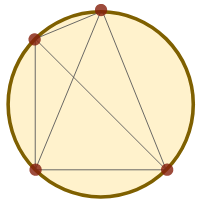
\includegraphics[height=3cm]{cake-4}
                \caption{\emph{
                    With $n=4$ people, we make ${n\choose 2}=6$ cuts, which gives
                    $8$ pieces in total ($4$ outside and $4$ inside).  
                }}
            \end{figure}

            Here are some drawings for possibilities ranging from $n=1$ people
            to $n=6$ people.  Try counting the pieces and guessing a pattern!
            Can you find a formula for how many pieces arise when there are $n$
            people?
            \begin{figure}[h!]
                \centering
                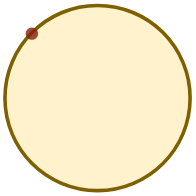
\includegraphics[height=3cm]{cake-1}
                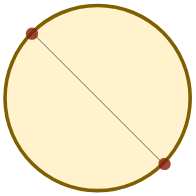
\includegraphics[height=3cm]{cake-2}
                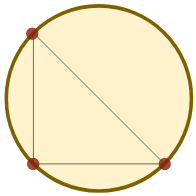
\includegraphics[height=3cm]{cake-3} \\
                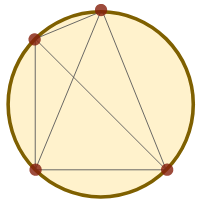
\includegraphics[height=3cm]{cake-4}
                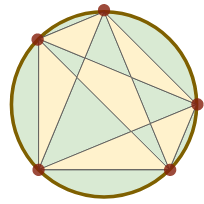
\includegraphics[height=3cm]{cake-5-col}
                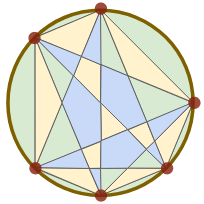
\includegraphics[height=3cm]{cake-6-col}
                \caption{\emph{
                    Here, we color some of the cake pieces just to make them
                    easier to see and to count.
                    %
                    The $n=1$ case doesn't have any cuts.
                    %
                    The $n=5$ case has $5$ outside green pieces, $5$ inside
                    green pieces, $5$ yellow triangles --- so far this is three
                    fives, which makes fifteen --- and what's left is $1$
                    yellow center piece.
                    %
                    The $n=6$ case has $6$ outside green pieces, $6$ inside
                    green pieces, $6$ outer yellow triangles, $6$ blue
                    triangles --- so far this is four sixes, which makes twenty
                    four --- and what's left are the $7$ central blue and
                    yellow shapes.
                }}
            \end{figure}

            Well, it seems that with $n=1, 2, 3, 4$ people, there are $p(n) =
            1, 2, 4, 8$ pieces.  (Here, $p$ stands for ``pieces'', and we'll
            use this way of writing just to save time).  It seems that $p(n)$
            doubles for each next $n$, meaning that $p$ looks like powers of
            two.  In symbols, our guess is: $p(n) \stackrel{?}{=} 2^{n-1}$.

            Let's check this guess.  Does it continue to $n=5$?  We expect the
            next power of two, namely $8+8=16$.  And yes: $p(5)$ really is
            $16$!  How about $n=6$?  We expect $16+16=32$.  But --- uh oh! ---
            it seems that there are only $31$ pieces.  So the pattern breaks.

        \subsection{An Explanation}
            Let's now figure out $p(n)$ for any $n$; along the way, we'll see
            why the powers-of-two pattern seemed to work until $n=6$.
            %
            There are two steps: we'll relate cake to constellations
            and then relate constellations to counting.

            We'll use Euler's polyhedron formula.  This formula says that if we
            connect a bunch of dots by edges to form some enclosed regions,
            then the numbers of dots, edges, and regions are related:
            $$
                \text{Regions} - \text{Edges} + \text{Dots} = 1
            $$
            For example, the constellation that we build up in stages below
            has $3$ regions (one pentagon and two triangles), $13$ edges, and
            $11$ dots.  And $3-13+11 = 1$, just like the formula says.
            %
            \begin{figure}[h!]
                \centering
                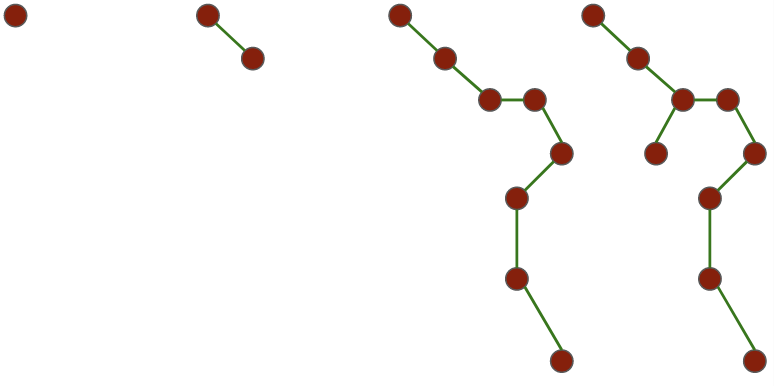
\includegraphics[height=3cm]{euler-a}
                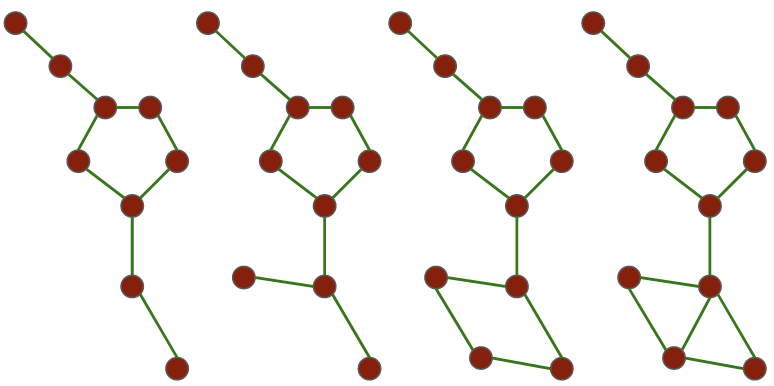
\includegraphics[height=3cm]{euler-b}
                \caption{\emph{
                    Steps to build an example constellation (right) starting
                    from a single dot (left).
                    %
                    By the way, this method only helps us build constellations
                    that don't have crossing edges, and each two of whose dots
                    are connected by a path of edges.  Euler's formula only
                    applies to constellations that follow these rules.
                }}
            \end{figure}
            %
            Why is the formula true?  Well, we can build up our constellation
            starting from a single dot.  The single dot follows the formula
            (since there are no regions and no edges, and $0-0+1 = 1$).  And
            each step of building preserves the formula:
            %
            \textbf{either} we connect a new dot to an old dot (so both
            $-\text{Edges}$ and $+\text{Dots}$ change by one, meaning that the
            total stays the same)
            %
            \textbf{or} we connect two old dots to create a new region (so both
            $\text{Regions}$ and $-\text{Edges}$ change by one, meaning that
            the total stays the same).  This logic proves Euler's formula. 

            To wrap up, let's think of a cake as a constellation as shown
            below.  In addition to $n$ outer dots, there are ${n \choose 4}$
            inner dots, because from each inner dot emanate $4$ rays pointing
            toward $4$ outer dots.  By similar logic, the number of edges is $n
            + 2{n\choose 2}/2 + 4{n \choose 4}/2$, since there are $n$ outer
            arcs (green), $2{n\choose 2}$ straight-half edges (blue) between
            outer dots, and $4$ half-edges (orange) emanating from each of
            ${n\choose 4}$ inner dots.
            %
            \begin{figure}[h!]
                \centering
                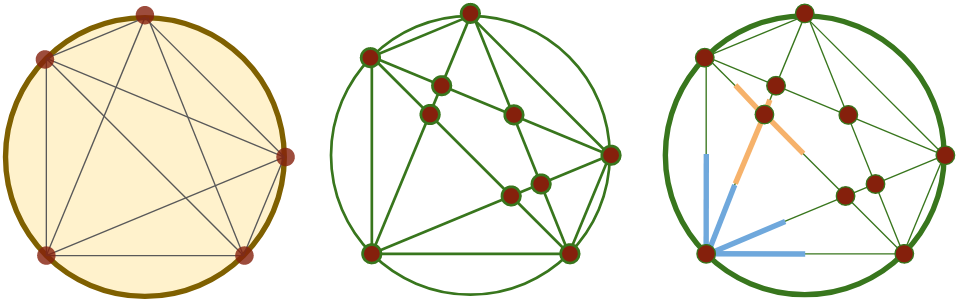
\includegraphics[height=3cm]{count}
                \caption{\emph{
                    We can think of a cake (left)
                    as a constellation (middle) by adding inner dots.
                    We can count the half-edges of the constellation (right) 
                    by binning them into three groups: the outer arcs (green),
                    the straight half-edges between outer dots (blue), and the
                    straight half-edges emanating from inner dots (orange).
                }}
            \end{figure}

            Putting all the pieces together, we find that
            $
                \text{Regions} = 1 + \text{Edges} - \text{Dots}
                               = 1 + {n\choose 2} + {n\choose 4}
            $.  We can simplify this by using the facts that $1={n-1 \choose
            0}$ and ${n \choose k} = {n-1 \choose k-1} + {n-1 \choose k}$:
            \begin{align*}
                \text{Regions}
                              = {n-1 \choose 0}
                              + {n-1 \choose 1}
                              + {n-1 \choose 2}
                              + {n-1 \choose 3}
                              + {n-1 \choose 4}
            \end{align*}
            %
            Since ${n-1\choose 0} + \cdots + {n-1\choose k} = 2^{n-1}$ as long
            as $k\leq n-1$, this looks like powers of two as long as $n\leq 5$.  
            %
            So we have solved the mystery.  With $n$ people, the number $p(n)$
            of pieces equals the number of subsets of people with at most $4$
            members.  Ain't that cool?  
 
    \section{Finite Hypothesis Classes}
        \subsection{What is Learning?}
            Today, we'll analyze machines that learn to classify images into
            two possible buckets such as Cow and Dog.  Most of our discussion
            extends to the case where there are more than two buckets and to
            other more complicated situations.  But we'll just focus on the
            simple case.  

            To use math, we need to precisely set up what we mean by ``machine
            learning''.  Here's how we'll do it in this class: we posit a set
            $\Xx$ of all possible images, a set $\Yy=\{\text{Cow},\text{Dog}\}$
            of buckets, and a probability distribution $\Dd$ over $\Xx \times
            \Yy$.  The distribution $\Dd$ models the world by telling us which
            pairs $(x,y)\in \Xx\times \Yy$ are more likely and which are less
            likely.  For instance: we might have $\sdia{cow-a},
            \sdia{cow-d},\cdots \in \Xx$, and $\Dd$ might say that
            $(\sdia{cow-a}, \text{Cow})$ is more likely to occur in nature than 
            $(\sdia{cow-d}, \text{Cow})$, which is more likely to occur than
            $(\sdia{cow-d}, \text{Dog})$, which in turn is more likely than
            to occur in nature than
            $(\sdia{cow-a}, \text{Dog})$.

            So far, we've given names $\Xx, \Yy, \Dd$ to aspects of the world.
            What's cool is that we don't have to know $\Dd$ in order for our
            mathematical theory to work!  We gave it a name just so we can
            reason about it.  While $\Dd$ models the world, we'd like our
            machine to learn by pondering finitely many sample pairs drawn from
            $\Dd$.  It's like learning which way a die is loaded by throwing it
            a hundred times and tabulating the results.  So we posit a set
            $\Hh$ of functions from $\Xx$ to $\Yy$.  Each function is one
            possible way of classifying images, and $\Hh$ is a set of many such
            functions.  We call these functions \textbf{hypotheses}, since we
            don't know which ones are good.  
            %
            As an example, $\Hh$ might have just three elements:
            \begin{align*}
                \Hh = \{
                    &\text{always say Cow}, \\
                    &\text{say Cow if $x$ is brown on average; otherwise, say Dog}, \\
                    &\text{say Cow if $x \in \{\sdia{cow-b}, \sdia{cow-c}, \sdia{cow-e}\}$;
                        otherwise, say Dog}
                \}
            \end{align*}
            In practice, $\Hh$ will actually be something like a set of neural
            networks, which is effectively an infinite set.

            A \textbf{learner} is then a rule $\Ll$ that assigns --- to each
            length-$N$ sequence $\Ss = ((x_i, y_i): 0\leq i<N)$ of samples ---
            a hypothesis $\Ll(\Ss) \in \Hh$.
            %
            A learner $\Ll$ is good when $\Ll(\Ss)$ classifies images
            accurately.  We mean not just the images (in $\Ss$) that we learned
            from; we want $\Ll$ to accurately classify new images freshly drawn
            from $\Dd$!  More formally, we define the \textbf{out-error} and
            \textbf{in-error} of a hypothesis $f \in \Hh$ as
            $$
                \Ee_{\text{out}}(f) = \PP_{(x,y)\sim\Dd}   
                                        \left[
                                            f(x) \neq y
                                        \right]
                ~~~~~~~~~~
                \Ee_{\text{in},\Ss}(f) = \PP_{(x,y)\sim\Ss}   
                                       \left[
                                           f(x) \neq y
                                       \right]
            $$
            Likewise, the out- and in-errors of a learner are
            $
                \Ee_{\cdots}(\Ll) = \EE_{\Ss\sim\Dd} \left[
                                        \Ee_{\cdots}(\Ll(\Ss)) 
                                    \right]
            $.
            We want $\Ee_{\text{out}}(f)$ to be low, but we can only directly
            calculate $\Ee_{\text{in}}(f)$, since we have access to the samples
            $\Ss$ but not the full distribution $\Dd$.

            Based on the intuition that $\Ee_{\text{out}}(f)$ and
            $\Ee_{\text{in},\Ss}(f)$ look similar, we propose a special learner
            $\Ll$ that works like this: compute the in-error
            $\Ee_{\text{in},\Ss}(f)$ for each $f\in \Hh$, and (breaking ties
            arbitrarily) settle on whichever $f$ has the smallest in-error.
            This heuristic is called \textbf{empirical risk minimization}, and
            its variants dominate modern machine learning.

            But does this special learner $\Ll$ actually work?  In particular,
            if $\Ee_{\text{in},\Ss}(\Ll)$ is small, will
            $\Ee_{\text{out}}(\Ll)$ also be small?  This is the question of
            \textbf{generalization}.

            Here's an example where the answer is yes.
                Imagine that there's one hypothesis $f\in \Hh$ (so $|\Hh| = 1$)
                and $N=10000$ datapoints.  Then $\Ee_{\cdots}(\Ll) =
                \Ee_{\cdots}(f)$, and by the law of large numbers
                $\Ee_{in,\Ss}(f)$ will with high probability be very close to
                $\Ee_{out}(f)$.

            Here's an example where the answer is no.
                Imagine that every possible function is in $\Hh$ (so $\Hh$ is
                very infinite), but only $N=3$ datapoints.  For any fixed $\Ss$,
                many hypotheses will have the same $\Ee_{\in,\Ss}$
                (pigeonhole).  Suppose $\Ll$ breaks ties in favor of
                memorizing; that is, $\Ll$ always settles on the hypothesis,
                $$
                    f(x) = \text{say Cow if $(x,\text{Cow}) \in \Ss$;
                            otherwise, say Dog}
                $$
                Then $f$ may have $\Ee_{\text{in},\Ss}(f)=0$, but unless the exact 
                images in $\Ss$ were extremely common, or unless most mammals
                are Dogs, $f$ will have $\Ee_{\text{out}}(f)\approx 1$.

            Intuitively, when $\Hh$ contains many hypothesis,
            generalization is difficult, and when the number $N$ of datapoints
            is large, generalization is easy.  How do these conflicting forces
            balance?  Let's use math to find out.

        \subsection{Is Learning Possible?}

    \section{Infinite Hypothesis Classes}
        \subsection{}
        \subsection{}
    
\end{document}
